\documentclass{article}
\usepackage[margin=1in]{geometry}  % set the margins to 1in on all sides
\usepackage{graphicx}              % to include figures
\usepackage{epstopdf}
\usepackage{amsmath}               % great math stuff
\usepackage{amsfonts}              % for blackboard bold, etc
\usepackage{amsthm}                % better theorem environments
\usepackage{amssymb}
\usepackage[english]{babel}
\usepackage[utf8]{inputenc}
\usepackage{fancyhdr}
\usepackage{tikz}
\usepackage{lipsum,array,amsmath}
\usetikzlibrary{positioning,automata}
\usetikzlibrary{arrows.meta}
\usepackage{pgfplots}
\usepackage{amsmath}
\DeclareMathOperator*{\argmax}{argmax}
\DeclareMathOperator*{\argmin}{argmin}
\usepackage{hyperref}
\usepackage{caption}
\usepackage{subcaption}
\usepackage{float}
\usepackage{algorithm,algorithmic}
\usepackage{bbold}
\usepackage{tabularx}
\usepackage{mathtools}


\pagestyle{fancy}
\fancyhf{}
\rhead{Islam A. Ali}
\lhead{CMPUT-566: Probabilistic Graphical Models}
\rfoot{Page \thepage}
\lfoot{\scriptsize{}}


\begin{document}


% =================== Header ====================
\begin{center}
{\bf CMPUT 566: Introduction to Machine Learning}  \\
{A Self-Study Report on: Probabilistic Graphical Models (PGMs)} \\
\vspace{.1in}
{\em Islam A. Ali}\\
{\em Student ID: 1633813}\\
{\em iaali@ualberta.ca}\\
\end{center}
\noindent\rule{\textwidth}{1pt}
% ==========================================================================

\section*{Abstract}
Abstract goes here 

\noindent\rule{\textwidth}{1pt}
% ==========================================================================
% Report Body
\section{What are Probabilistic Graphical Models (PGMs)?}
Probabilistic Graphical Models (PGMs) are statistical model that can be used to represent complex dependencies between random variables efficiently using graphs data structure. This dependencies are modeled as joint distributions. However, with the increase of the number of random variables involved, the need to have a more efficient way of representation is needed. The graph representation provide efficiency in terms of time complexity as well as scale-ability to more complex systems as it models random variables and the conditional dependencies among them allowing for scale-ability in terms of problems studied.
\section{Motivation}
To motivate the idea of having a more complexity-efficient statistical model for dependencies representation, an example of industrial defects in products diagnosis system is discussed. Let's say a product in a production line can either be malfunctioned electrically or mechanically or both. This can be represented by a joint distribution of two random variables where each is representing a certain malfunction. Further, we can expand the diagnosis system to the reason for defect. For instance in the electrical defects, it is because of PCBs manufacturing or due to components defects, on the other hand, the mechanical malfunction can be either from the material used or the methodology utilized. And the relations goes on, with extended number of random variables, that can be very expensive to represent or to query using regular mathematical methods. In this case, the rise of the PGMs makes sense, where such a system can be represented as a graph with nodes representing each random variable in the system, and with directed edges representing the dependencies and their directions. \\
\indent Other motivation comes from the graph theory itself, where a wide range of research was done and was proven to be correct for data dependency representation, query, and manipulation. A wide range of efficient algorithms are available for all these purposes and even beyond.
% ==========================================================================
\section{Mathematical Background}
In this section, we briefly review the main concepts that will be used throughout this report. For this purpose, a review of both probability theory and the graph theory are reviewed briefly by mentioning their most famous/important rules and concepts. This quick review intentions is to act as a reminder and not an extensive review of theories. 
\subsection{Probability Theory}
Probability theory's main objective is to systematically study uncertainty or the degree of confidence in quantities or measurements. The following are the three main axioms of probability:
\begin{enumerate}
 \item \textbf{Sample Space:} It is the set of all possible outcomes of a certain experiments, it is denoted by $\Omega$.
 \item \textbf{Event Space:} It is a subset of the sample space and represents a limited set of possible outcomes of the experiment, it is denoted by $\digamma$.
 \item \textbf{Probability Measure:} It is a measure that maps the event space to real numbers, it is denoted by $P$, and it satisfies a number of rules:
 	\begin{itemize}
 	\item $P(A) \geq 0 $
 	\item $P(\Omega) = 1$
 	\item The union of disjoint events is the summation of their probabilities.
 	\end{itemize}
\end{enumerate} 

\subsubsection{Conditional Probability and Independence}
The conditional probability is the probability of the occurrence of an event after observing another event. This is given by the following formula:
\begin{equation}
P(A|B) = \frac{P(A \cap B)}{P(B)}
\end{equation}
Independence, on the other hand, is mainly defined as the first event having no impact on the second event and can be mathematically represented as:
\begin{equation}
P(A \cap B) = P(A)P(B)
\end{equation}

\subsubsection{Results of Conditional Probability: Chain Rule and Bayes Rule}
Based on the conditional probability, we can deduce the following relation that is called the chain rule:
\begin{equation}
P(A \cap B) = P(A|B) P(B)
\end{equation}
More generally, if a series of events $A_1, A_2, ..., A_n$, the probability of a certain event can be given by:
\begin{equation}
P(A_1 \cap ... \cap A_n) = P(A_1)P(A_1|A_2) ... P(A_1|A_2 \cap ... \cap A_n)
\end{equation}
Another result of the conditional probability, is the Bayes Rule which allows to compute a certain conditional probability from its inverse with some knowledge of probability priors. The mathematical representation is defined as:
\begin{equation}
P(A|B) = \frac{P(B|A)P(A)}{P(B)}
\end{equation}

\subsubsection{Random Variables, Marginal, and Joint Distributions}
A random variable is defined by a function that assigns a value for all possible outcome of a certain measurable experiment. It is a very useful when dealing with complex and dependent relations of events where each has its own probabilistic properties. \\ 
One of the associated concepts to random variables is marginal distribution. The marginal distribution of random variable $X$ is defined as the distribution over the events in which $X$ is involved, and is denoted by $P(X)$. Another concept associated with random variable is joint distributions, which is defined as the distribution over events in which two or more random variables are involved, and is denoted by $P(X,Y)$. It can also be mathematically represented by:
\begin{equation}
P_{XY}(x,y) = P_{XY}(y|x)P_Y(x)
\end{equation}

\subsubsection{Mean/Expectation and Variance}
Two other concepts related to probability theory are mean and variance which can be used to describe a probability distribution. The mathematical formula for the expectation in both the discrete and continuous cases are given by:
\begin{equation}
\mathbb{E} [X] = \sum_x x.P(x)
\end{equation}
\begin{equation}
\mathbb{E} [X] = \int_x x.P(x) \; dx
\end{equation}
While the variance is defined as: 
\begin{equation}
\mathbb{V}ar [X] = \mathbb{E} [X^2] - \mathbb{E}^2 [X]
\end{equation}
% ==========================================================================
\subsection{Graph Theory}
A graph is a data structure that is structured from two elements that are: nodes and edges. It is mainly used to represented relations between generic data elements via connections among nodes via edges. Graphs can have multiple structure and can be categorized based on many aspects such as:
\begin{enumerate}
\item What nodes represent?
\item Is it a directed or undirected graph?
\item Is it a fully or partially directed graph?
\item Are the edges weighted or not?
\item Are cycles and loops allowed or not?
\item What are the traversal techniques allowed?
\end{enumerate}
In the context of this report, nodes represent random variables while edges represent the relations/dependency/conditional relationship between random variables. Edges in this context can either be directed or undirected, and can allow loops and cycles. The following is an example of a directed graph \footnote{Image was downloaded from: \url{https://computersciencewiki.org/index.php/The_web_as_a_directed_grap}}:
\begin{figure}[H]
\centering
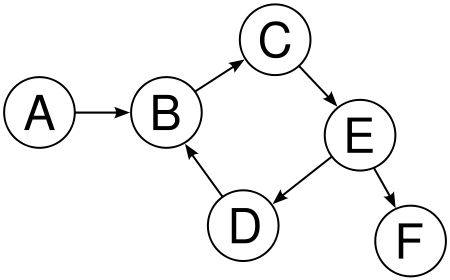
\includegraphics[width=0.4\textwidth]{Directed_graph.png}
\caption{Example of Directed Graph }
\end{figure}
% ==========================================================================

\section{PGMs Representation}
PGMs has many representations such as \textit{Bayesian Networks} where edges are directed and are indicated by an arrow in the graphical representation. Another type is the \textit{Markov Random Fields} in which edges are undirected and are represented by lines. The first method is useful for conditional dependency representation, while later one is useful in representing soft constraints. In this report, we focus on directed probabilistic graphical models, known as \textbf{"Bayesian Networks"}.
\subsection{Bayesian Networks Representation}
Bayesian Networks, a.k.a Bayesian Belief Networks (BBNs), are PGMs that represent the conditional relations between random variables by directed acyclic graph (DAG). \\
Formally, a Bayesian Network $BN$ is represented by:
\begin{equation}
BN = (g, \{ P{X_1},..., P{X_N}  \})
\end{equation}
\textbf{Where:} $g$ is a directed acyclic graph (DAG) represented as $g=(X,E)$. From the definition of the DAG, $X$ are the graph nodes representing random variables, while $E$ are the edges connecting nodes to each other representing conditional independence between random variables. $P{X_1},..., P{X_N}$ are the conditional probability distributions associated with each node/random variable. It is represented as a table indicating the relations between ancestors of a certain node and the resulting probability for each outcome of the same node. In the following diagrams we present the probability distribution table associated with a certain node in the BN context.

\begin{figure}[H]
	\centering
	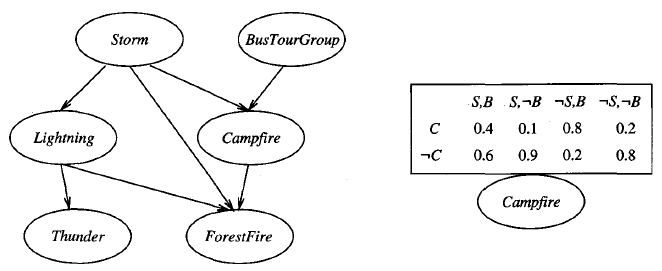
\includegraphics[width=0.8\textwidth]{cond_prob.png}
	\caption{BN with Conditional Probability Table}
\end{figure}
For the sake of formulation, we also define the parameter $\Theta = \{\theta_1, ..., \theta_k\}$, which are the parameters which define the probability distribution for each node. For instance, in case of a Gaussian distribution, for the node $X_i$, the set of parameters defining it are given by: 
\begin{equation}
\Theta_i = (\mu_i, \sigma_i)
\end{equation}
\textbf{Where:} $\mu_i$ and $\sigma_i^2$ are the mean and variance of the Gaussian distribution describing node $X_i$. Accordingly, the BN can be defined in terms of the parameters defining the probability distributions as follows:
\begin{equation}
BN = (g, \{ \Theta_1,..., \Theta_N  \})
\end{equation}
It worth mentioning that in some of the references, the parameter $\Theta$ refers to the weights and bias for each probability distribution rather than the mean and variance or the parameters defining the distribution. The definition of weight and bias and their impact on the distributions are not provided, unless they refer to the weight and bias governing the mean definition, which will then make $\Theta=(w_i, b_i, \sigma_i)$. 

\subsubsection{Factorization Properties}
The factorization property allow for defining the joint distribution as a multiplication of conditional probabilities governed by the conditional independence implied in the graph structure. Each of the conditional probability distributions are denoted by:
\begin{equation}
P_{X_i} = (X_i | P_g (Xi))
\end{equation}
Which means that the probability of a certain random variable is defined by the conditional probability relative to its parents/ancestors in the DAG. \\
Based on the previous relation and the definition of a joint probability given in the introduction, the complete joint probability of the BN $P_{BN}(X_i, ..., X_N)$ (Where N is the number of random variable in the BN), is given by:
\begin{equation}
P_{BN}(X_i, ..., X_N) = \prod_{i=1}^{N} (X_i | {Parent}_g (Xi))
\end{equation}
Applying this rule on the example BN given in Fig. 2, we can end up with the following joint distribution (note that for each node, the initials are used as random variable names. e.g. Storm --> S).
\begin{equation}
P_{BN}(X_i, ..., X_N) = P(S).P(B).P(L|S).P(C|S,B).P(T|L).P(F|L,S,C)
\end{equation}
Based on the joint distribution factorization, one can easily proof that conditional probability in case of parameters independence. For this, we seek to get the conditional probability of a certain node given all other node available in the graph. For example, we seek to get $P(C|S,B, L, T, F)$ in the previously mentioned example in Fig. 2. According to the relation between conditional probability and the factorization principle illustrated, the conditional probability can be re-written as:
\begin{equation}
P(C|S,B, L, T, F) = \frac{P(C,S,B,L,T,F)}{P(S,B,L,T,F)}
\end{equation}
The joint distributions can be further expanded as:
\begin{equation}
P(C,S,B,L,T,F) = P(S)P(B)P(L|S)P(C|S,B)P(T|L)P(F|L,S,C)
\end{equation}
\begin{equation}
P(S,B,L,T,F) = \sum_{C} P(C,S,B,L,T,F)
\end{equation}
\begin{equation}
P(S,B,L,T,F) = \sum_{C} P(S)P(B)P(L|S)P(C|S,B)P(T|L)P(F|L,S,C)
\end{equation}
\begin{equation}
P(S,B,L,T,F) = P(S)P(B)P(L|S)(\sum_{C}P(C|S,B))P(T|L)P(F|L,S,C)
\end{equation}
The summation over all values of a random variable =1, from the basic probability axioms, which imply:
\begin{equation}
P(S,B,L,T,F) = P(S)P(B)P(L|S)P(T|L)P(F|L,S,C)
\end{equation}
Therefore, the conditional probability can be re-written as:
\begin{equation}
P(C|S,B, L, T, F) = \frac{P(S)P(B)P(L|S)P(C|S,B)P(T|L)P(F|L,S,C)}{P(S)P(B)P(L|S)P(T|L)P(F|L,S,C)}
\end{equation}
After canceling out equal terms in the fraction, we end up with:
\begin{equation}
P(C|S,B, L, T, F) = P(C|S,B)
\end{equation}
Which imply the independence of the node of any non-parent node. 

\subsubsection{Conditional Independence Property}
Conditional independence is a very important property when dealing with BNs that can substantially simplify the structure of the joint distributions and can provide a concise presentation of it when factorized. As suggested by the literature, conditional independence is considered the backbone of BNs due to the face that the structure of the graph and the complexity reduction advantage are mainly basing on this property. \\
Consider the case when we have a BN with three nodes, where nodes c->a and c->b are connected. The independence of random variable $a$ and $b$ are coming from the definition of the c and its relation to both random variables. The following is the definition of conditional independence:
\begin{equation}
P(a,b|c) = P(a|c)P(b|C)
\end{equation}
In this case, $a$ and $b$ are declared conditionally independent given $c$ and this can be denoted by the perpendicular sign $\perp$ such that:
\begin{equation}
P(a \perp b |c) = P(a|c)
\end{equation}
\begin{equation}
P(b \perp a |c) = P(b|c)
\end{equation}
This definition stems from the definition of the joint distribution of independent random variables given by (in case of $a$ and $b$ begin independent):
\begin{equation}
P(a,b) = P(a)P(b)
\end{equation} 
Alternatively, the definition of conditional independence can be given by:
\begin{equation}
P(a|b,c) = P(a|c)
\end{equation}
The proof for this relation comes from the joint distribution definition and its relation to the conditional probability definition, and it goes as follows:
\begin{equation}
P(a|b,c) = \frac{P(a,b,c)}{P(b,c)}
\end{equation}
\begin{equation}
P(a|b,c) = \frac{P(a,b|c)P(c)}{P(b|c)P(c)}
\end{equation}
From the first definition of conditional independence:
\begin{equation}
P(a|b,c) = \frac{P(a|c)P(b|c) P(c)}{P(b|c)P(c)}
\end{equation}
Canceling out equivalent terms:
\begin{equation}
P(a|b,c) = P(a|c)
\end{equation}
To show the impact of the conditional independence on the complexity reduction, we consider the following network structure. Assume we have $n=20$ binary random variables, with a structure having each node in the network to have a maximum of 4 parent nodes. The number of probability values needed to be calculated in order to decide on an outcome in case of having no conditional independence assumption is given by:
\begin{equation}
count(P)_{total} = 2^{n} = 2^{20}
\end{equation}
While in case of utilizing the reduction from the conditional independence the number goes down to:
\begin{equation}
count(P)_{total} = n*(2^k) = 20*(2^4)= 20*16= 320 \approxeq 2^9
\end{equation}
Which is a huge improvement in terms of complexity.
\subsubsection{Proof for The Conditional Independence Property}
In order to prove the conditional independence property, we define three types of nodes with respect to a certain $X_i$ node:
\begin{enumerate}
\item Descendant Node: Which is one of the children of $X_i$, either directly or non-directly.
\item Parent Node: Which are nodes having $X_i$ as one of their descendants.
\item Non Descendant Node: Which are node that are neither descendants nor parents.
\end{enumerate}
Intuitively, a node have dependency on descent node, then the following relation is sufficient to prove the conditional dependency:
\begin{equation}
P(X_i|non-desc(X_i),Parent(X_i)) = P(X_i|Parent(X_i)) 
\end{equation} 
Again, using the joint probability and the relation to conditional probability, we get:
\begin{equation}
P(X_i|non-desc(X_i),Parent(X_i)) = \frac{P(X_i, non-desc(X_i), Parent(X_i))}{P(non-desc(X_i)P(Parent(Xi)))}
\end{equation}
\begin{equation}
numerator = \sum_{desc(X_i)} P(X_i, non-desc(X_i), Parent(X_i), desc(X_i))
\end{equation}
Which can be factorized based on each node type as follows:
\begin{equation}
= \sum_{desc(X_i)} (P(X_i|Parent(X_i)))*(\prod_{\mathclap{X_j \in desc(X_i)}} P(X_j|Parent(X_j)))*(\prod_{\mathclap{X_k \in {non-desc(X_i) \bigcup parent(X_i)}}} P(X_k|Parent(X_k)))
\end{equation}
Given the fact that the summation over all values of desc = 1 from the prob. axioms, the numerator can be reduced to:
\begin{equation}
= (P(X_i|Parent(X_i))) \sum_{desc(X_i)}\;\;\;\;\;\;\;\;\;\;\;\;\;\;\;\;\;\;\;\;(\prod_{\mathclap{X_k \in {non-desc(X_i) \bigcup parent(X_i)}}} P(X_k|Parent(X_k)))
\end{equation}
Processing the denominator will be as follows:
\begin{equation}
denominator = \sum_{desc(X_i)}\;\;\;\;\;\;\;\;\;\;\;\;\;\;\;\;\;\;\;\ (\prod_{\mathclap{X_k \in {non-desc(X_i) \bigcup parent(X_i)}}} P(X_k|Parent(X_k)))
\end{equation}  
by dividing the above two equations, we get the final formula as:
\begin{equation}
P(X_i|non-desc(X_i),Parent(X_i)) = P(X_i|Parent(X_i)) 
\end{equation} 
Which proves the conditional independence property.
% ==========================================================================
\section{Learning in PGMs}
After illustrating the representation of BNs, and the significance of their usage in machine learning problems, the learning process of this model is now discussed. The objective of the learning process it to have a BN that we can use to get the probability distribution of a random variable over all possible values of this variable. In this context we do have three cases as follows:
\begin{enumerate}
\item Both BN structure and conditional probabilities are known, and in this case, the inference process is straight forward. 
\item Only the structure of the BN is known, and the conditional probabilities are not defined. In this case, The learning process would be to define the probability distribution tables associated with each random variable. In this stated that, domain experts may define the optimal structure of the BN but the training data may not have enough observability over internal random variables.
\item Both the structure and the conditional probabilities are not known and the objective of the training process is to determine both the optimal structure and the conditional distributions given the training data. 
\end{enumerate}
In all cases, the learning process will depend on the the specific task and the available knowledge of the system and whether the domain experts are available for providing the optimal structure of the BN. Additionally, it worth mentioning that having a full automated model that can learn both the structure of the network and the probability distributions and the conditional relations is the optimal case and the ultimate objective in learning PGMs.
\subsection{Learning The Conditional Distribution Tables of BNs}
In the case where the structure of the network is defined, meaning that for each random variable/node in the BN $X_i$; the parents $Parent(X_i)$ and descendants $Desc(X_i)$ of this random variables $X_i$ are defined and the conditional independences are known. In this case, we assume partial observability of conditional distribution tables associated with each node. In this section, we discuss the Gradient Ascent Algorithm that can be used to learn the entries of the tables given the structure and partial observability. From an abstract point of view, the algorithm depends on searching in hypotheses $H$ and tries to maximize $P(D|h)$, where $D$ is the available training data, and $h$ is one hypothesis in the hypothesis space. More formally, we need to define the following terms:
\begin{itemize}
\item $P(D|h)$: is the probability of the training data given a certain hypothesis
\item $d \in D$: is a data sample inside the training data, the training data $D$ is of size $M$.
\item $w_{ijk}$: is an entry in one of the conditional distribution tables associated with each random variable $Y_i$.
\item $Y_{i}$: is the random variable in hand to which the table is being calculated.
\item $U_{i}$: is the set of parent nodes for the random variable $Y_i$.
\item $y_{ij}$: is one value of possible values for random variable $Y_i$.
\item $u_{ik}$: is one value of possible values for parent $U_k$ or random variable $Y_i$.
\end{itemize}


\subsection{Hyperparameters}
\section{Inference in PGMs}
\section{Applications/Examples}
\section{State-of-the-art Work}
\section*{Discussion}
% ==========================================================================
\section*{Conclusion}
% ==========================================================================
\nocite{cs229}
\nocite{koller2009probabilistic}
\nocite{pernkopf2014introduction}
\nocite{bishop2006pattern}
\nocite{mitchell1997machine}
\nocite{kimArticle}
\bibliographystyle{ieeetr}
\bibliography{refs}
% ==========================================================================
\end{document}